\chapter{State of the art}
In the introduction chapters, a overview and definition of VR was given. The reader was able to get a small insight in the world of virtual reality. The following chapter will deepen the knowledge in VR and related technologies. Some basic concept about virtual reality will be explained. Later on there will be a summary of the latest state of research. Current VR related hardware devices as well as software applications will be presented. It will also be pointed out, of what VR is not capable yet. The aim of this chapter is to get an overview about the topic of VR and the state of research as it is for now.
\section{VR basic concepts}
\todo{covering some history in this chapter too? E.g. explaining the first wave of VR in the 90s}
\cite{Sherman.2019} describe five core concepts for virtual reality.  According to them, this concepts are the key elements when it comes to design a virtual reality. In the following, this concepts will be explained:
\paragraph{Participants} A participant is a user of a VR application, who is actually wearing the HMD and experiencing the virtual world. Every participant has a different perception of the application, so every experience can be seen as a unique experience. This is because the several participants differ from their cultural background, their age, their expectations and their knowledge in technology. Therefore, it is a challenge for developers of VR applications to provide a virtual world in which various users can feel comfortable. The role of the participants is described as the most important role by \cite{Sherman.2019}, because all the experience is happening in their imagination. Developers or creators are only capable of creating the framework around the experience.
\paragraph{Creators} Creators or developers design and implement a VR application for participants. As mentioned, the developers are not able to create the experience of the users. The core aim of their work is to develop the application, which is a collection of programming scripts, concept designs and data. Together with the participants the experience is created. The following chapters design and implementation (TODO ref) will take a look at the VR application from a creator's perspective, whilst chapter (TODO ref) will dive into the different experiences of participants using the VR application.
\paragraph{Virtual world} In general, the term "virtual world" is defined as the content of a virtual reality application.  The virtual world is the skeleton of the virtual experience. Precisely, it is a description of the objects inside the virtual space. TODO schwammig

\paragraph{Immersion} Immersion in general describes, how deeply users connect to a virutal world. They experience something through a medium which they would not be able to experience without it. They see actions and things through a different point of view and can connect to it in some way. The deeper a user can connect to the virtual environment and the objects inside it, the more immerse the VR experience is for them. In chapter \ref{chap:Immersion and storytelling} the term immersion will be explained in more detail.

\paragraph{Interaction} Most of the time, interaction means a manipulation of a computer generated world. However, interaction can also happen in a non artificial environment. An example for this are interactive novels, or text based computer games. In this mediums/media?, computer graphics are not required and yet they provide a form of user interaction. When it comes to VR, interaction also means relocating a viewport inside a virutal world. Participants can move physically in the virtual environment. Another form of interaction is the collaborative interaction. In some VR applications it is not only possible to interact with the virtual world but also to share the space with other participants and interact with them. This can be in a virtual or physical way.
\subsection{Different dimensions of reality}
\todo{describe different states: reality, augmented reality, augmented virtuality, vr}
Despites VR, there exist other technologies, which serve the purpose to create a virtual world for the user. They differ in the extend of intervention with the reality. \cite{Tham.2018} show a spectrum of different types of technologies and their dimension of reality. A visual representation of this spectrum is displayed in \ref{fig:spectrum}.\\
\begin{figure}[h!]
  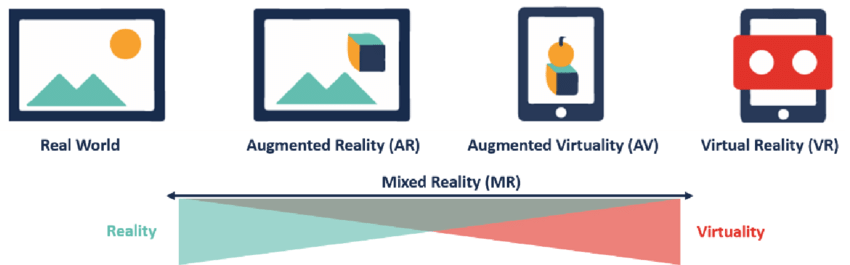
\includegraphics[width=14cm]{kapitel/spectrum-of-reality.png}
  \centering
  \caption{Graphical representation of the dimensions of reality by 	  \cite{Lovreglio.2018}}
  \label{fig:spectrum}
\end{figure}

The reality describes the real world and using non digital devices to interact with it, such as a steering wheel for driving a car for example. As already mentioned in the indroduction, AR is a related technology to VR. In the spectrum of \cite{Tham.2018} augmented reality covers the second level of reality dimensions. It describes computer generated elements, which are embedded into the reality. A famous example for a AR application is the game PokemonGo (TODO source), in which players search in the real environment for computer generated items, based on a phone's camera and location services. The next level of reality is the augmented virtuality. This preamble describes a virtual environment, in which users can interact through analogue methods. An example for this could be a video chat room where the participants are present in a virtual room but communicate through analogue methods. As seen in figure \ref{fig:spectrum}, augmented reality and augmented virtuality can be summed up with the term \"mixed reality\" which describes the interaction between real life elements and the virtual environment. Finally, in the last stage is the virtual reality in which a user is fully surrounded by a computer generated environment. This environment is most likely a reproduction of a real-life environment. The user is not only surrounded by an artificial reality but can also interact with it. It might appear that the user actually feels present in the virtual reality. In the following, this phenomenon will be explained in more detail.

\subsection{Immersion and storytelling}
\todo{What is immersion and why so important for VR? What describes a good storytelling? Is there anything special when designing a story for a VR application?}
The term immersion often comes up when talking about VR. As mentioned before, this term describes a experience which users would not be able to percieve without the use of a medium. In general, it describes a experience from a different point of view. This could be for example the story of a different character or the exploration of a unknown location. \cite{Tham.2018} \\
When talking about immersion, it is important to distinguish between two types: mental and physical immersion. Mental immersion is when the participant feels deeply emotionally connected to the virtual world. Physical immersion on the other hand means that the user's physical interactions are transferred into the virtual environment with the use of technology. When talking about immersion in books, films or related media, it is often only referred to mental immersion, because these types of media are not able to provide the technology for interacting with their environments. VR on the other hand can create immersion through a physical way as well. That is why VR can provide a higher grade of immersion than other media. \cite{Tham.2018}\\
Another term closely related to immersion is presence. Presence in the context of VR describes a subjective feeling of participants to actually exist in the virtual world. The feeling of presence is a mix between mental and physical immersion. The more presence user feel, the more they accept the virtual world as the reality. To gain the sense of presence, the participant's movements in the reality should match with the movements of the virtual world. With a higher grade of presence, participants act more natural in a virutal environment, such as they would in a real environment. Through this, their task performance increases. This is one reason why presence is an important factor when it comes to developing VR, especially in the field of education and learning. \cite{Slater.1997}\\

Since the terms immersion and presence are explained, it is now the question, how design the story of a VR application in order to gain a maximum grade of immersion. Storytelling is one of the most important elements for mental immersion in a virtual experience. Especially mental immersion can be influenced by the storyline, while physical immersion can be increased through hardware tools. \\
Storytelling in general is the art of telling a narrative to the user in a way that the user is not only consumer but actually feels immersed with the story.\cite{Louden.2018}. Designing a storyline in VR opens a lot of possibilities in engaging the participant in the story. Therefore there are things to consider when it comes to storytelling in VR: \cite{Keane.2018}\\
One thing to bear in mind is, that space and environment in a VR application are more important than in other media, like books or films. The creator designs a world in a 360 degree view, so there is a lot more space to show. The storyline not only happens in front of the users, but can be all around them. Because the user can walk freely around in the virtual world, it is very important to softly guide the user into a certain direction when necessary for the storyline. The guidance should not be conspicuous, but should attract the users curiosity. This can be achieved through light and sound effects or movements. Another aspect to consider is not to overwhelm the user with complex tasks. This could prevent the user in experiencing an immersed virtual world because their full attention would lie on completing the tasks.
\subsection{Interaction: Selection and manipulation in VR}
\section{Hardware for VR}
\todo{describe difference between mobile and desktop HMDs, show examples HTC Vive and Google Daydream, maybe also Google Cardboard. What possibilities of interaction do they provide?}
\section{Showcases of VR applications}

\section{Limits of VR}
\todo{At current status, what is VR not able to achieve? What are the challenges VR researchers face currently?}